\documentclass[bwprint]{gmcmthesis}
\usepackage[framemethod=TikZ]{mdframed}
\title{高压油管稳定控压策略的研究}
\baominghao{22103350008} %参赛队号
\schoolname{浙江大学}%学校名称
\membera{葛明阳} %队员A
\memberb{郑欣怡} %队员B
\memberc{董萌苇} %队员C
\begin{document}
\sloppy

 %生成标题
 \maketitle

 %填写摘要
\begin{abstract}
本文对高压油管、高压油泵和喷啧啧啧嘴口建立\textbf{微分模型},通过数值解法得到高压油管的油压变化,并通过设定优化目标,建立规划问题。使用\textbf{优先搜索、控制变量、稀疏遍历}等算法提高求解问题的速度与精度。同时,也对模型中主要参数进行了灵敏度分析,将主要参数设置到合适的数值。
\keywords{混合整数线性规划;混合整数非线性规划;粒子群算法;FFF;贪婪;BL;优先搜索;}
\end{abstract}

%\pagestyle{plain}
%目录 不推荐加
%\tableofcontents

\section{问题重述}
\subsection{问题背景}

方形件产品(也称板式类产品)是一类以板材为主要原片、经平面加工后组合装配形成的产品,如3C(计算、通讯、消费电子)、板式家具、玻璃、钣金件等。因其“多品种小批量”的个性化定制生产模式,企业通常需要进行订单组批和排样优化,降低原材料消耗,保证生产效率。

\textbf{订单组批}是指针对数量庞大的不同订单,将其组成若干批次,实现批量化生产。批次的定义为完成若干订单全部任务且不含任何不完整订单任务的订单集合。订单组批时,通常会将具有相同材质、交货期相近、工艺相似的订单安排在同一个生产批次。

\textbf{排样优化}是指合理规划方形件在板材原片上的布局,最大化材料利用率,简化切割过程。切割工艺根据是否任何一次直线切割都能保证板材可分离可分为齐头切和非齐头切,齐头切又可根据是否在有限切割阶段数内切割出准确尺寸的方形件分为精确方式和非精确方式。以3个阶段的切割方式为例,第1阶段切割生成模块可称为stripe(条带),第2阶段切割生成模块可称为stack(栈),第3阶段生成模块可称为item(产品项)。

\quad
\subsection{问题提出}
基于上述问题背景,根据题目提供的输入参数(包括单个批次产品项总数上限和面积总和上限、原片长度和宽度)和产品项数据集(包括产品项材质、数量、长度、宽度和订单号),完成下述两个问题:

\textbf{子问题1},考虑相同材质的产品项,忽略订单组批过程,在采用齐头切的三阶段精确排样方式下,给出产品项排样方法,将所有产品项排样,得到板材用量最少(即板材利用率最高)的排样方案。并利用数据集A对排样方法加以验证,将数据集A的排样结果以表格、示意图的形式进行展示描述。最后,对排样方法进行评价。

\textbf{子问题2},在问题1的基础上,解决订单组批问题。在具有不同材质、不同订单号、不同产品项大小的情况下。考虑同一订单产品项全部在同一批次、同一材质产品项方可使用同一板材原片、每个批次产品项总数和面积总和均不超过上线的约束,采用齐头切的三阶段精确排样方式,给出组批方法,得到总板材用量最少的订单组批方案及相应各批次排样方案。并利用数据集B加以验证,将数据集B的组批和排样结果以表格、示意图的形式进行展示描述,并对组批方法进行评价。

\newpage
\section{模型假设}


(1) 只考虑齐头切的切割方式(直线切割、切割方向垂直于板材一条边,并保证每次直线切割板材可分离成两块);

(2) 切割阶段数不超过3,同一个阶段切割方向相同;

(3) 排样方式为精确排样;

(4) 假定板材原片仅有一种规格且数量充足;

(5) 排样方案不用考虑锯缝宽度(即切割的缝隙宽度)影响;

(6)所有订单的交货期均相同。

\quad
\section{符号说明}
{\centering
\newcommand{\tabincell}[2]{\begin{tabular}{@{}#1@{}}#2\end{tabular}}
\begin{tabular}{cccc}
 \hline
  \makebox[0.05\textwidth][c]{序号}  &  \makebox[0.2\textwidth][c]{符号}	&  \makebox[0.65\textwidth][c]{意义} \\ \hline
  1 & $n$            & 产品项总个数      \\ 
  1 & $i$            & 产品项编号($i\le n,i \in \mathbb{N}^+$)      \\ 
  1 & $j$            & 栈编号($j\le n,j \in \mathbb{N}^+$)      \\ 
  1 & $k$            & 条带编号($k\le n,k \in \mathbb{N}^+$)      \\ 
  1 & $l$            & 板材原片编号 ($l\le n,l \in \mathbb{N}^+$)     \\ 
  2 & $Item_{i}$     & 编号为$i$的产品项	  \\ 
  3 & $Stack_{j}$    & 编号为$j$的个栈       \\ 
  4 & $Stripe_{k}$   & 编号为$k$的条带	  \\ 
  5 & $Bin_{l}$      & 编号为$l$的板材原片  \\ 
  6 & $h_{i}$      & 产品项$Item_i$的高度(单位:mm) \\ 
  7 & $w_{i}$      & 产品项$Item_i$的宽度(单位:mm) \\ 
  8 & $H$          & 板材原片的高度(单位:mm)\\ 
  9 & $W$          & 板材原片的宽度(单位:mm) \\ 
  10 & $a_{j,i}$    & 标志$Stack_j$是否包含$Item_i$的0-1变量  	&\quad   \\  
  11 & $b_{k,j}$    & 标志$Stripe_k$是否包含$Stack_j$的0-1变量 	&\quad   \\  
  12 & $r_{l,k}$    & 标志$Bin_l$是否包含$Stripe_k$的0-1变量  	&\quad   \\  \hline
\end{tabular}
}
\newpage

\section{问题一排样优化}

\subsection{问题分析}
问题一解决同一批次产品项的排样优化问题,优化目标是尽可能减少板材用量,即板材原片使用的块数最少,约束条件

目标函数和约束条件是待求变量的线性函数
指全部决策变量都必须取整数值
模型中的所有变量均为整数,建立整数线性规划模型

属于一个规则物体的二维裁剪问题。裁剪问题,可以转化为将若干个较小的二维图形,分组不重叠的拼接成若干个较大的二维图形,在每个拼接生成的二维图形外边界均不超过规定尺寸的前提下,分组数尽可能少的组合和拼接方案。
对于本题而言,
是将各给定尺寸的矩形产品项按照最佳的布局方式排入若干块大的原料板材中以最大化材料利用率。而对裁剪方式的规定,及

不妨设




\subsubsection{决策变量}
定义标志各产品项、栈、条带、板材原片之间包含关系的决策变量如下:
\begin{equation}   %\mbox{中文}
    a_{j,i}=
    \begin{cases}
        1, \quad  & Item_i \in  Stack_j \\
        0,\quad  & Item_i  \notin  Stack_j \\
    \end{cases}
\end{equation}

\begin{equation}
    b_{k,j}=
    \begin{cases}
        1, \quad  & Stack_j \in  Stripe_k \\
        0,\quad  & Stack_j  \notin  Stripe_k \\
    \end{cases}
\end{equation}

\begin{equation}
    r_{l,k}=
    \begin{cases}
        1, \quad  & Stripe_k \in  Bin_l \\
        0,\quad  & Stripe_k  \notin  Bin_l \\
    \end{cases}
\end{equation}

\subsubsection{编号规则}

(1)\textbf{产品项}:将各个产品项按长度从大到小排序后,从1到n依次编号;

(2)\textbf{栈}:用栈中包含产品项的最小编号为该栈编号,若1到n中还有剩余编号,则这些编号分别对应一个不包含任何产品项、也不包含于任何条带的空栈;

(3) \textbf{条带}:用条带中包含栈的最小编号为该条带编号,若1到n中还有剩余编号,则这些编号分别对应一个不包含任何栈、也不包含于任何板材原片的空条带;

(4)\textbf{板材原片}:用板材原片中包含条带的最小编号为该板材原片编号,若1到n中还有剩余编号,则这些编号分别对应一个不包含任何条带(未使用)的空板材原片。

根据上述编号规则,可知
% (这里注意要不要写成约束)

\begin{equation}
    h_{1} \ge h_{2} \ge ... \ge h_{n}
\end{equation} 
\begin{equation}
    a_{j,i}=0, \quad   j>i
\end{equation}
\begin{equation}
    b_{k,j}=0, \quad   k>j
\end{equation}
\begin{equation}
    r_{l,k}=0, \quad   l>k
\end{equation}
\begin{equation}
    a_{j,j}=
    \begin{cases}
        1, \quad  & Stack_j \neq  \phi  \\
        0,\quad  & Stack_j  =  \phi  \\
    \end{cases}
\end{equation}
\begin{equation}
    b_{k,k}=
    \begin{cases}
        1, \quad  & Stripe_k \neq  \phi  \\
        0,\quad  & Stripe_k =  \phi  \\
    \end{cases}
\end{equation}
\begin{equation}
    r_{l,l}=
    \begin{cases}
        1, \quad  & Bin_l \neq  \phi  \\
        0,\quad  & Bin_l = \phi  \\
    \end{cases}
\end{equation}


\subsubsection{方向说明}
为了便于后续讨论,本文规定第一阶段切割方向为x方向,垂直切割方向

垂直于高度、平行于长度的方向,如图\ref{方向说明1}、图\ref{方向说明2},才
为了便于后续讨论,如图将第一阶段切割方向规定为横切,与之垂直的板材原片的边的长度规定为板材原片的高度H,平行的边的长度规定为板材原片的长度D。
\begin{figure}[!htbp]
    \centering
    \begin{minipage}{0.48\linewidth}
        \centering
        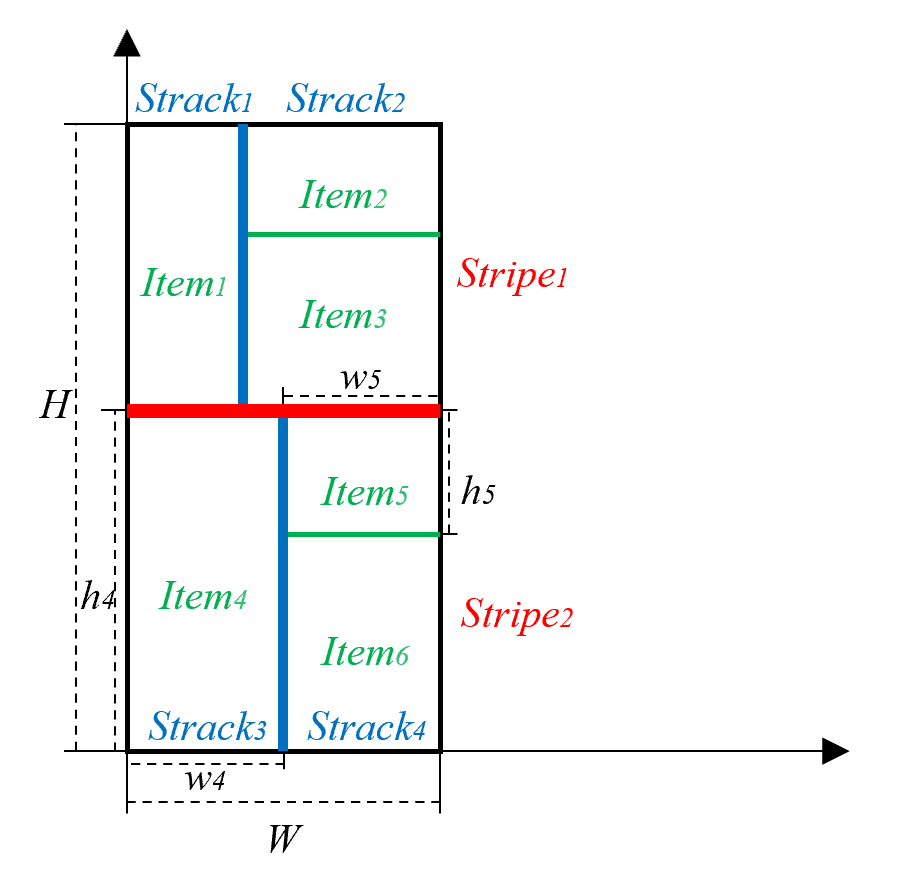
\includegraphics[width=.9\textwidth]{方向说明1.png}
        \caption{排布方案方向一}\label{方向说明1}
    \end{minipage}
    \begin{minipage}{0.48\linewidth}
        \centering
        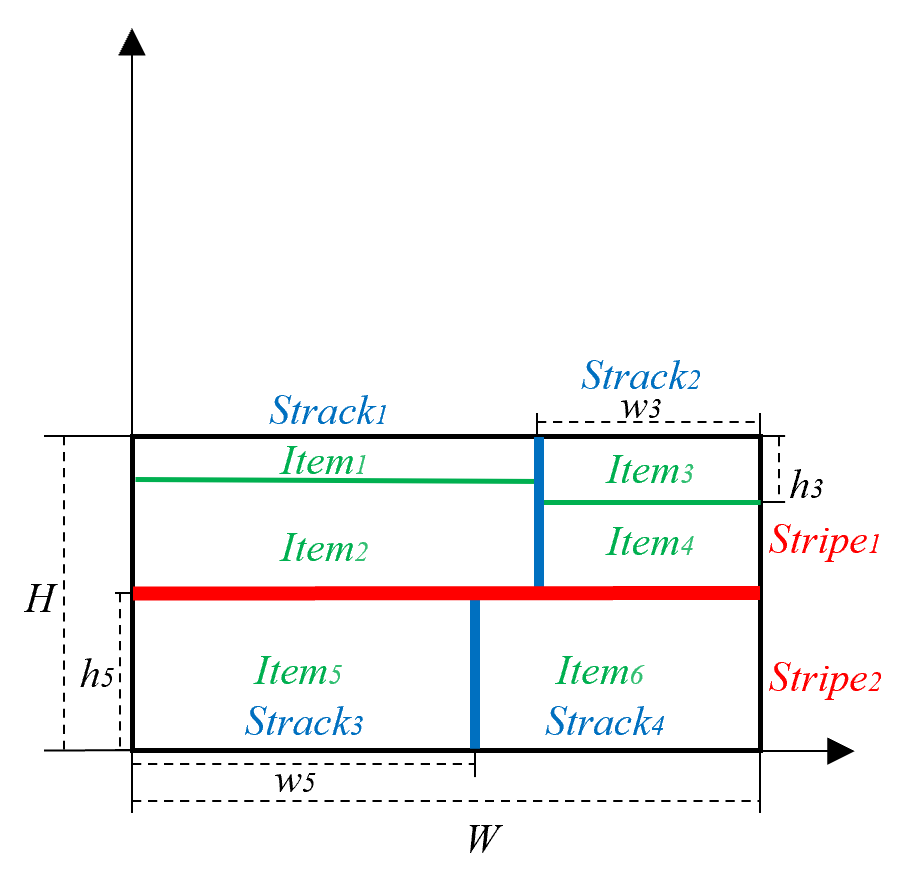
\includegraphics[width=.9\textwidth]{方向说明2.png}
        \caption{排布方案方向二}\label{方向说明2}
    \end{minipage}
\end{figure}

\begin{figure}[!htbp]
        \centering
        \includegraphics{Batch1-Board1-MaterialYW10-0218S.png}
        \caption{排布方案方向一}
\end{figure}


\subsubsection{目标函数}
最小化板材原片使用数量:
\begin{equation}
    Min \sum_{l=1}^{n} r_{l,l} 
\end{equation}

\subsubsection{约束条件}
每个产品项当且仅当出现在一个栈中
\begin{equation}
    \sum_{j=1}^{n} a_{j,i}=\sum_{j=1}^{i} a_{j,i}=1
\end{equation}  

而每个非空栈当且仅当出现在一个条带中
\begin{equation}
    \sum_{k=1}^{n} b_{k,j}=\sum_{k=1}^{j} b_{k,j}=a_{j,j}
\end{equation}  

同理

\begin{equation}
    \sum_{l=1}^{n} r_{l,k}=\sum_{l=1}^{k} r_{l,k} =b_{k,k}
\end{equation}  

\begin{equation}
    \sum_{i=1}^{n} r_{j,i}=1
\end{equation}  


\begin{equation}
    a_{j,i}=0, \quad   h_{i}+h_{j}>H
\end{equation}
\begin{equation}
    a_{j,i}=0, \quad  w_{i} \ne w_{j}
\end{equation}


\begin{equation}
    a_{j,j}=1
\end{equation}


\begin{equation}
    b_{k,k}=1
\end{equation}

\begin{equation}
    r_{l,l}=1
\end{equation}












相同栈里的产品项宽度或长度相同
\begin{equation}
    \sum_{l=1}^{k} a_{l,k}=1,\quad \forall k\leqslant n
\end{equation}  

\subsection{模型建立}
通过前述问题分析,我们建立了如下数学模型:




\begin{equation}
    \begin{aligned}
    Min \sum_{l=1}^{n} r_{l,l}\\
    Min \sum_{l=1}^{n} r_{l,l}
    \end{aligned}
\end{equation}  





\begin{equation}
    \begin{aligned}
    Min \sum_{l=1}^{n} r_{l,l}\\
    Min \sum_{l=1}^{n} r_{l,l}
    \end{aligned}
\end{equation}  




\subsubsection{条件限制}


根据每次切割均必须垂直于板材边界,易知对于统一板材而言切割只有垂直于高或者垂直于宽两种方向,且各个阶段的切割方向交替进行,即第一阶段与第三阶段切割方向一致,第二阶段切割方向垂直于第一和第三阶段。为便于后续讨论,我们不妨规定在第一阶段完成尽可能多的切割。







此外,不妨规定每个条带中包含的长度最大的条带始终由单个产品项组成。



综上,针对问题一排布优化建立的\textbf{整数线性规划模型}如下:



\section{备用}
信号干扰下的超宽带(UWB)精确定位问题,是指考虑\textbf{信号干扰}的前提下,利用基于飞行时间(Time of Flignt,TOF)测距原理的UWB定位技术,采集锚点(anchor)与靶点(Tag)之间的距离,确定Tag的精确定位(3维坐标)。

\textbf{任务1},对在场景1:$5000mm*3000mm*3000mm$测试环境范围内324个不同位置Tag,分别在信号干扰和信号无干扰下接收4个角落anchor信号,所解算出的距离数据文件,考虑在同一位置连续时间中自动采集多组数据、采集异常等问题,进行数据预处理,最终对每个位置Tag只保留有效采集的信号干扰和信号无干扰下各一组数据。

\textbf{任务2},分别利用经任务1处理的信号无干扰下的“正常数据”和信号干扰下的“异常数据”,求解各个位置Tag的精确定位(3维坐标)。

\textbf{任务3},对在场景2:$5000mm*3000mm*3000mm$测试环境范围内,5个Tag在信号干扰、5个Tag在信号无干扰下接收4个位置anchor信号,所解算出的距离数据,求解相应位置Tag的精确定位(3维坐标)。

\textbf{任务4},提出一种判断数据是在信号有无干扰的情况下采集的方法,并使用场景1经任务1处理后的数据和场景2数据进行验证。

\textbf{任务5},根据一段时间内连续采集动态靶点的多组数据,判断各组数据是在信号有无干扰的情况下采集,并分别求解相应Tag的精确定位,结合靶点自身运动规律画出运动轨迹。

\subsection{引言}
创意平板折叠桌注重于表达木制品的优雅和设计师所想要强调的自动化与功能性。为了增大有效使用面积。设计师以长方形木板的宽为直径截取了一个圆形作为桌面,又将木板剩余的面积切割成了若干个长短不一的木条,每根木条的长度为平板宽到圆上一点的距离,分别用两根钢筋贯穿两侧的木条,使用者只需提起木板的两侧,便可以在重力的作用下达到自动升起的效果,相互对称的木条宛如下垂的桌布,精密的制作工艺配以质朴的木材,让这件工艺品看起来就像是工业革命时期的机器。

\subsection{问题的提出}

\subsubsection{问题的提出内容一}

(1) 围绕创意平板折叠桌的动态变化过程、设计加工参数,本文依次提出如下问题:
给定长方形平板尺寸 ($120 cm \times 50 cm \times 3 cm$),每根木条宽度(2.5cm),连接桌腿木条的钢筋的位置,折叠后桌子的高度(53 cm)。要求建立模型描述此折叠桌的动态变化过程,并在此基础上给出此折叠桌的设计加工参数和桌脚边缘线的数学描述。

(2)折叠桌的设计应做到产品稳固性好、加工方便、用材最少。对于任意给定的折叠桌高度和圆形桌面直径的设计要求,讨论长方形平板材料和折叠桌的最优设计加工参数,例如,平板尺寸、钢筋位置、开槽长度等。对于桌高70 cm,桌面直径80 cm的情形,确定最优设计加工参数。

(3)给出软件设计的数学模型,可以根据客户任意设定的折叠桌高度、桌面边缘线的形状大小和桌脚边缘线的大致形状,给出所需平板材料的形状尺寸和切实可行的最优设计加工参数,使得生产的折叠桌尽可能接近客户所期望的形状,并根据所建立的模型给出几个设计的创意平板折叠桌。要求给出相应的设计加工参数,画出至少8张动态变化过程的示意图。


\section{模型的假设}

\begin{itemize}
\item 忽略实际加工误差对设计的影响;\cite{wright_latex3_2009}
\item 木条与圆桌面之间的交接处缝隙较小,可忽略;
\item 钢筋强度足够大,不弯曲;
\item 假设地面平整。
\end{itemize}

\section{符号说明}
\begin{tabular}{cccc}
 \hline
  \makebox[0.12\textwidth][c]{序号}  &  \makebox[0.12\textwidth][c]{符号}	&  \makebox[0.5\textwidth][c]{意义} &\makebox[0.2\textwidth][c]{单位}\\ \hline
 1 & D    & 木条宽度(cm)   &cm\\ 
 1 & L   & 木板长度(cm)	 &cm \\ 
 1 & W   & 木板宽度(cm)	 &cm \\ 
 1 & N	    & 第n根木条	   &cm \\ 
 1 & T	    & 木条根数	   &cm \\ 
 1 & H	    & 桌子高度(cm)	 &cm \\ 
 1 & R	    & 桌子半径(cm)	  &cm\\ \hline
 1 & R	    & 桌子直径(cm)	 &cm \\ \hline
\end{tabular}


\section{问题qqQQAAAAaaaAAAAAAAAAAAAAAAAA}
\section{问题分析}

\subsection{问题一分析}
题目要求建立模型描述折叠桌的动态变化图,由于在折叠时用力大小的不同,我们不能描述在某一时刻折叠桌的具体形态,但我们可以用每根木条的角度变化来描述折叠桌的动态变化。首先,我们知道折叠桌前后左右对称,我们可以运用几何知识求出四分之一木条的角度变化。最后,根据初始时刻和最终形态两种状态求出桌腿木条开槽的长度。
$$\pi\times$$
\begin{equation}
\pi\times
\end{equation}


\subsection{问题二分析}
题目要求从折叠桌的稳固性好、加工方便、用材最少三个角度,确定设计加工参数。我们可以从应力、支撑面积考虑稳固性,从开槽长度考虑加工方便,从木板长度考虑用材最少。而它们之间又是相互制约,我们需要确定最优设计加工参数,可以建立非线性规划模型,用lingo软件来求解最优设计加工参数(平板尺寸、钢筋位置、开槽长度等),这里以合力的方向(斜向上)与最长木条(桌腿)的夹角方向最小为目标函数,以木条所承受应力小于木条的许用应力、支撑面积大于桌面面积、木条的开槽长度小于木条本身长为约束条件。图发发斯蒂芬打算\ref{asdf}

\begin{equation}
    f(x) = \begin{cases}
        \frac{1}{2} = 0.5 \\
        \frac{1}{2} = 0.5 \\
        \frac{2}{3}
    \end{cases}\label{asdf}
    \begin{matrix}
        1 && 2 && 3 \\
        4 && 5 && 6
    \end{matrix}
\end{equation}

\subsection{问题三分析}
题目要求制作软件的意思就是客户给定折叠桌高度、桌面边缘线的形状大小和桌脚边缘线的大致形状,将这些信息输入程序就得到客户想要的桌子。我们在求解最优设计加工参数时,自行给定桌面边缘线形状(椭圆、相交圆等),桌脚边缘线形状,折叠桌高度,应用第二问的非线性规划模型,用MATLAB软件绘制折叠桌截面图,得到自己设计的创意平板折叠桌。


\newpage
\quad
\newpage

%参考文献   手工录入
%\begin{thebibliography}{9}%宽度9
% \bibitem{bib:one} ....
% \bibitem{bib:two} ....
%\end{thebibliography}

%采用bibtex方案
\bibliographystyle{gmcm}
\bibliography{MCM_2022}

\cite{mittelbach_latex_2004,wright_latex3_2009,beeton_unicode_2008,vieth_experiences_2009}


\newpage
%附录
\appendix

%\setcounter{page}{1} %如果需要可以自行重置页码。
\section{数据预处理及读取函数}
\lstinputlisting[language=matlab]{../code/data_pre_fun.m}
\section{问题一主程序}
\lstinputlisting[language=matlab]{../code/q1_main.m}
\section{问题一FFF算法}
\lstinputlisting[language=matlab]{../code/q1_FFF_fun.m}
\section{问题二主程序}
\lstinputlisting[language=matlab]{../code/q2_main.m}
\section{问题二XX算法}
\lstinputlisting[language=matlab]{../code/q2_tanlan.m}
\section{将计算结果保存至文件}
\lstinputlisting[language=matlab]{../code/save_to_file_fun.m}
\section{绘制排样图至文件}
\lstinputlisting[language=matlab]{../code/draw_picture_fun.m}

\end{document} 